\section{Methods}\label{sec:method}
The goal is to adapt a pretrained VLA to complete language-conditioned manipulation tasks on a target robot without collecting human demonstrations. We study multi-stage pick-and-place tasks: an instruction such as \emph{put the apple on the plate} requires approach, grasp, lift, transport, and release. The policy receives camera images, proprioception, and an instruction, predicts an action chunk, and executes a prefix before observing again.

During acquisition, each skill has its own instruction, success condition, and starting states. During composition and final evaluation, the robot starts with an empty gripper and receives one complete-task instruction. This distinction prevents isolated skill performance from being treated as full-task success. Algorithm~\ref{alg:paper_pipeline} summarizes the pipeline: acquire simple skills, consolidate them, and learn the complete instruction.

We use SmolVLA as the pretrained model~\cite{smolvla}. On the CDPR and WidowX, we map its action prior to three translation commands, yaw, and gripper opening. A newly initialized residual MLP receives the mapped prior and observation features and predicts corrections to an eight-action chunk. The robot executes four actions before observing again. Earlier training also adapts the pretrained expert with low-rank adapters. The final stage freezes the expert and its adapters and continues training the retained residual controller.


\begin{algorithm}[!t]
\caption{Staged VLA adaptation}
\label{alg:paper_pipeline}
\small
\begin{algorithmic}[1]
\State Load the pretrained VLA, initialize the residual controller, and create successful-trajectory banks.
\State Train approach, pickup, and placement separately with dense rewards, using each skill's instruction and reset conditions.
\State After each skill, evaluate the earlier skills. If they have degraded, fit the shared policy to a balanced bank of earlier and recent successes and evaluate it again.
\State Refine the skills with binary completion rewards, repeating the retention checks and recovery when needed.
\State Relabel successful skill trajectories with the complete instruction. Collect compatible segments for composition and fit their actions under that instruction.
\State Train the complete task from empty-gripper starts with milestone feedback, and evaluate complete-task success.
\State If composition plateaus and the budget permits, freeze the VLA and its adapters, retain the learned residual, reset the optimizer, and continue full-task RL with the same milestone rewards. In the CDPR continuation, likelihoods are evaluated on stored pre-clipping samples conditional on their recorded episode offsets.
\end{algorithmic}
\end{algorithm}


\subsection{Obtaining the first successful attempts}\label{sec:skill_acquisition}
We start from simple skills which can be described with a dense reward that measures progress before successful completion. For each skill, we introduce a stepwise schedule that distances the robot's starting position from the successful completion of the task, provided that a certain success rate is achieved. For bowl placement on the CDPR, the distance cap increases from 0.10 to 0.13, 0.16, and 0.19 m. Together with DAPO-style dynamic sampling, this increases the opportunity to obtain informative sampled groups, without guaranteeing that every sampled group is informative.

For \emph{move to the apple}, progress is measured by the distance between the gripper and the object. For \emph{pick up the apple}, proximity, grasp, and lift distinguish an approach from a completed pickup. Placement starts with an already held object, so the robot can practice transport and release before it can reliably pick up the object itself. Dense rewards allow two failed attempts to contribute to an update when one makes more progress than the other. Once successful attempts are available, binary refinement rewards completion of the skill.
For a fixed scene, let $p$ be the probability of success on one attempt and $G$ the number of independent attempts in a group. A binary group is informative when it contains at least one success and one failure. Its probability is

\begin{equation}
P_{\mathrm{mixed}}=1-(1-p)^G-p^G.
\label{eq:mixed}
\end{equation}

The two subtracted terms are the probabilities that all attempts fail or all attempts succeed. At $p=0.03$ and $G=8$, only 21.6\% of groups contain both outcomes. Dynamic sampling filters uniform groups and collects additional groups within the rollout budget. With dense feedback, the filtering criterion is variation in return; with binary feedback, it is variation in success.

\begin{figure}[!htb]
\centering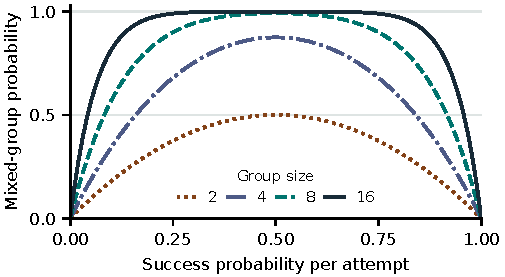
\includegraphics[width=0.95\columnwidth]{figures/mixed_groups.pdf}
\caption{Mixed-outcome probability for group sizes $G=2,4,8,16$. The curves describe independent binary attempts at a fixed scene.}
\label{fig:mixed}
\end{figure}

But the frequency of informative GRPO groups differs from average task success. The expected binary reward is $p$, whereas $P_{\mathrm{mixed}}$ is highest at $p=0.5$ and falls as success approaches one. With binary rewards, group normalization also changes how much each scene contributes to the expected on-policy GRPO update. When scenes share a policy, the resulting objective can favor a small gain in one scene over a larger loss in another~\cite[Sec.~6]{davis2025}.

For example, consider two equally likely scenes and groups of eight attempts. Suppose a policy change raises success in the first scene from 1\% to 2\% and lowers it in the second from 50\% to 48.8\%. The expected fraction of mixed groups rises from 53.47\% to 57.06\%, and the finite-group GRPO objective rises from 0.5381 to 0.5399. Mean task success falls from 25.5\% to 25.4\%.

The numbers illustrate the unfiltered on-policy binary-reward model in~\cite[Sec.~6]{davis2025} in the zero-stabilizer limit.


\label{sec:dense_method}
We also ran additional validations on LIBERO, comparing terminal-only, phase-only, and combined dense-and-phase rewards. These validations examine complete benchmark instructions. They do not directly measure the success of the separately trained skills in our adaptation pipeline. We will conduct more experiments which show separate skill success rates.

The combined LIBERO reward uses a manually defined sequence of reach, grasp, lift, move, and place phases. For each phase, a progress measure is normalized to the interval from zero to one. Reaching uses gripper--object distance, lifting uses height gained above the initial object position, and transport uses planar object--target distance. Grasping also uses gripper closure and grasp state; placement uses target proximity, release, and environment success. For current progress $q_t$ and the previous maximum $q_{\mathrm{best}}$, the rewarded increment is $\max(q_t-q_{\mathrm{best}},0)$. A completion predicate advances the tracker and adds a phase bonus. The bounded progress increment and phase bonus are combined with terminal feedback, while the native task-success verifier remains unchanged. The phase-only condition sets the continuous-progress weight to zero.

This reward construction requires a progress function, normalization, and relevant state variables for every phase. In our adaptation pipeline, we use dense feedback for the initial simple skills and reuse their binary completion predicates during full-task training.


\subsection{Retaining skills through self-imitation}\label{sec:retention_method}
After collecting successful trajectories for individual skills, we relabel them with a composed instruction and then start self-imitation learning---when the model learns on episodes generated by itself. We also smooth demonstrations with a moving average to get rid of sharp actions. Some demonstrations become unsuccessful; we remove them from the SIL bank. For the CDPR skill bank, the moving average spans five decisions. We replay the smoothed actions from the recorded reset and retain only trajectories which still satisfy the skill's success condition. The bank stores observations from replay together with the actions that produced them.

We balance earlier and recent successful trajectories by instruction. The supervised objective is the squared error between predicted and recorded actions. After fitting, we evaluate every skill again, because an improvement in placement can conceal a loss of pickup when only the average success rate is reported. The bank may contain trajectories from several earlier policies; it is not restricted to the current policy's latest episodes.

\subsection{Composing skills under one instruction}\label{sec:composition}
Relabeling changes the instruction associated with each segment. A reaching segment originally recorded under \emph{move to the apple} is then used to teach the same first movement under \emph{put the apple on the plate}. Concatenating segments additionally requires compatible states: pickup must begin where approach ended, and placement must begin with the grasp produced by pickup. In the CDPR experiments, we collected such segments with scripted assistance at skill transitions. Training also used complete demonstrations generated by a scripted simulator controller. These assisted and scripted data are distinguished from the policy's own unassisted successes.

For ordered skill-success events $E_1,\ldots,E_n$ under one instruction, the chain rule gives

\begin{equation}
P(\mathrm{complete})=\prod_{i=1}^{n}P(E_i\mid E_1,\ldots,E_{i-1}),
\label{eq:chain}
\end{equation}

where the first factor is $P(E_1)$. The placement factor therefore depends on the grasp actually produced during the episode. An isolated placement rate measured from a prepared grasp under a placement instruction cannot be substituted for this conditional probability. Self-imitation teaches the actions under the composed instruction, but does not guarantee a particular composed success rate.

\subsection{Learning from partial completion}\label{sec:milestones}
At the last training stage, we use a sparse phased reward based on the completion condition of each skill. During CDPR full-task RL, the first milestone requires reaching within 3 cm of the grasp point or establishing a grasp. The second requires a held lift of at least 5 cm. The third requires strict placement. The robot starts with an empty gripper and receives the complete instruction.

For eight attempts at the same scene, we compare outcomes separately at each milestone. Actions receive the group-relative advantage for their current stage. A successful placement also credits the earlier actions. When placement fails, an achieved approach or pickup keeps its local credit. For example, an attempt which lifts the apple and drops it and an attempt which never grasps it both fail the terminal test, but their pickup outcomes differ. A uniform placement outcome provides no local advantage for release. The WidowX implementation uses the fraction of milestones reached as its staged return.

The same distinction between informative groups and task success applies to each phase. A mixed pickup group provides a comparison for learning pickup, but does not by itself establish an improvement in complete-task success. We therefore report both milestone completion and the strict full-task result.
